%---------
\documentclass[12pt]{article}
\usepackage{graphicx}
\graphicspath{ {./images/} }

\title{Research Portfolio}
\author{Yuanshao Yang}


% -- START OF DOC -- % 
\begin{document}

\maketitle


\tableofcontents
\newpage

\section{Series Spring Design of Open-Source Leg}

\subsection{Background}

\subsection{Objectives}

\subsection{Results}


\section{Software Library Generalization for Open-Source Leg}


\subsection{Background}

% -- BACKGROUND BEGINS -- % 


Thus, a generalized, user-friendly version of the software library is needed to serve as a basis for alternative prosthetic leg forks. Such library will allow other researchers to fork their version of Open-Source Leg with lower costs and more standardized features, in order to offer a common platform for researchers to test and evaluate further control strategies and mechanical designs.

% -- BACKGROUND ENDS -- % 


\subsection{Objectives}

\subsection{Results}

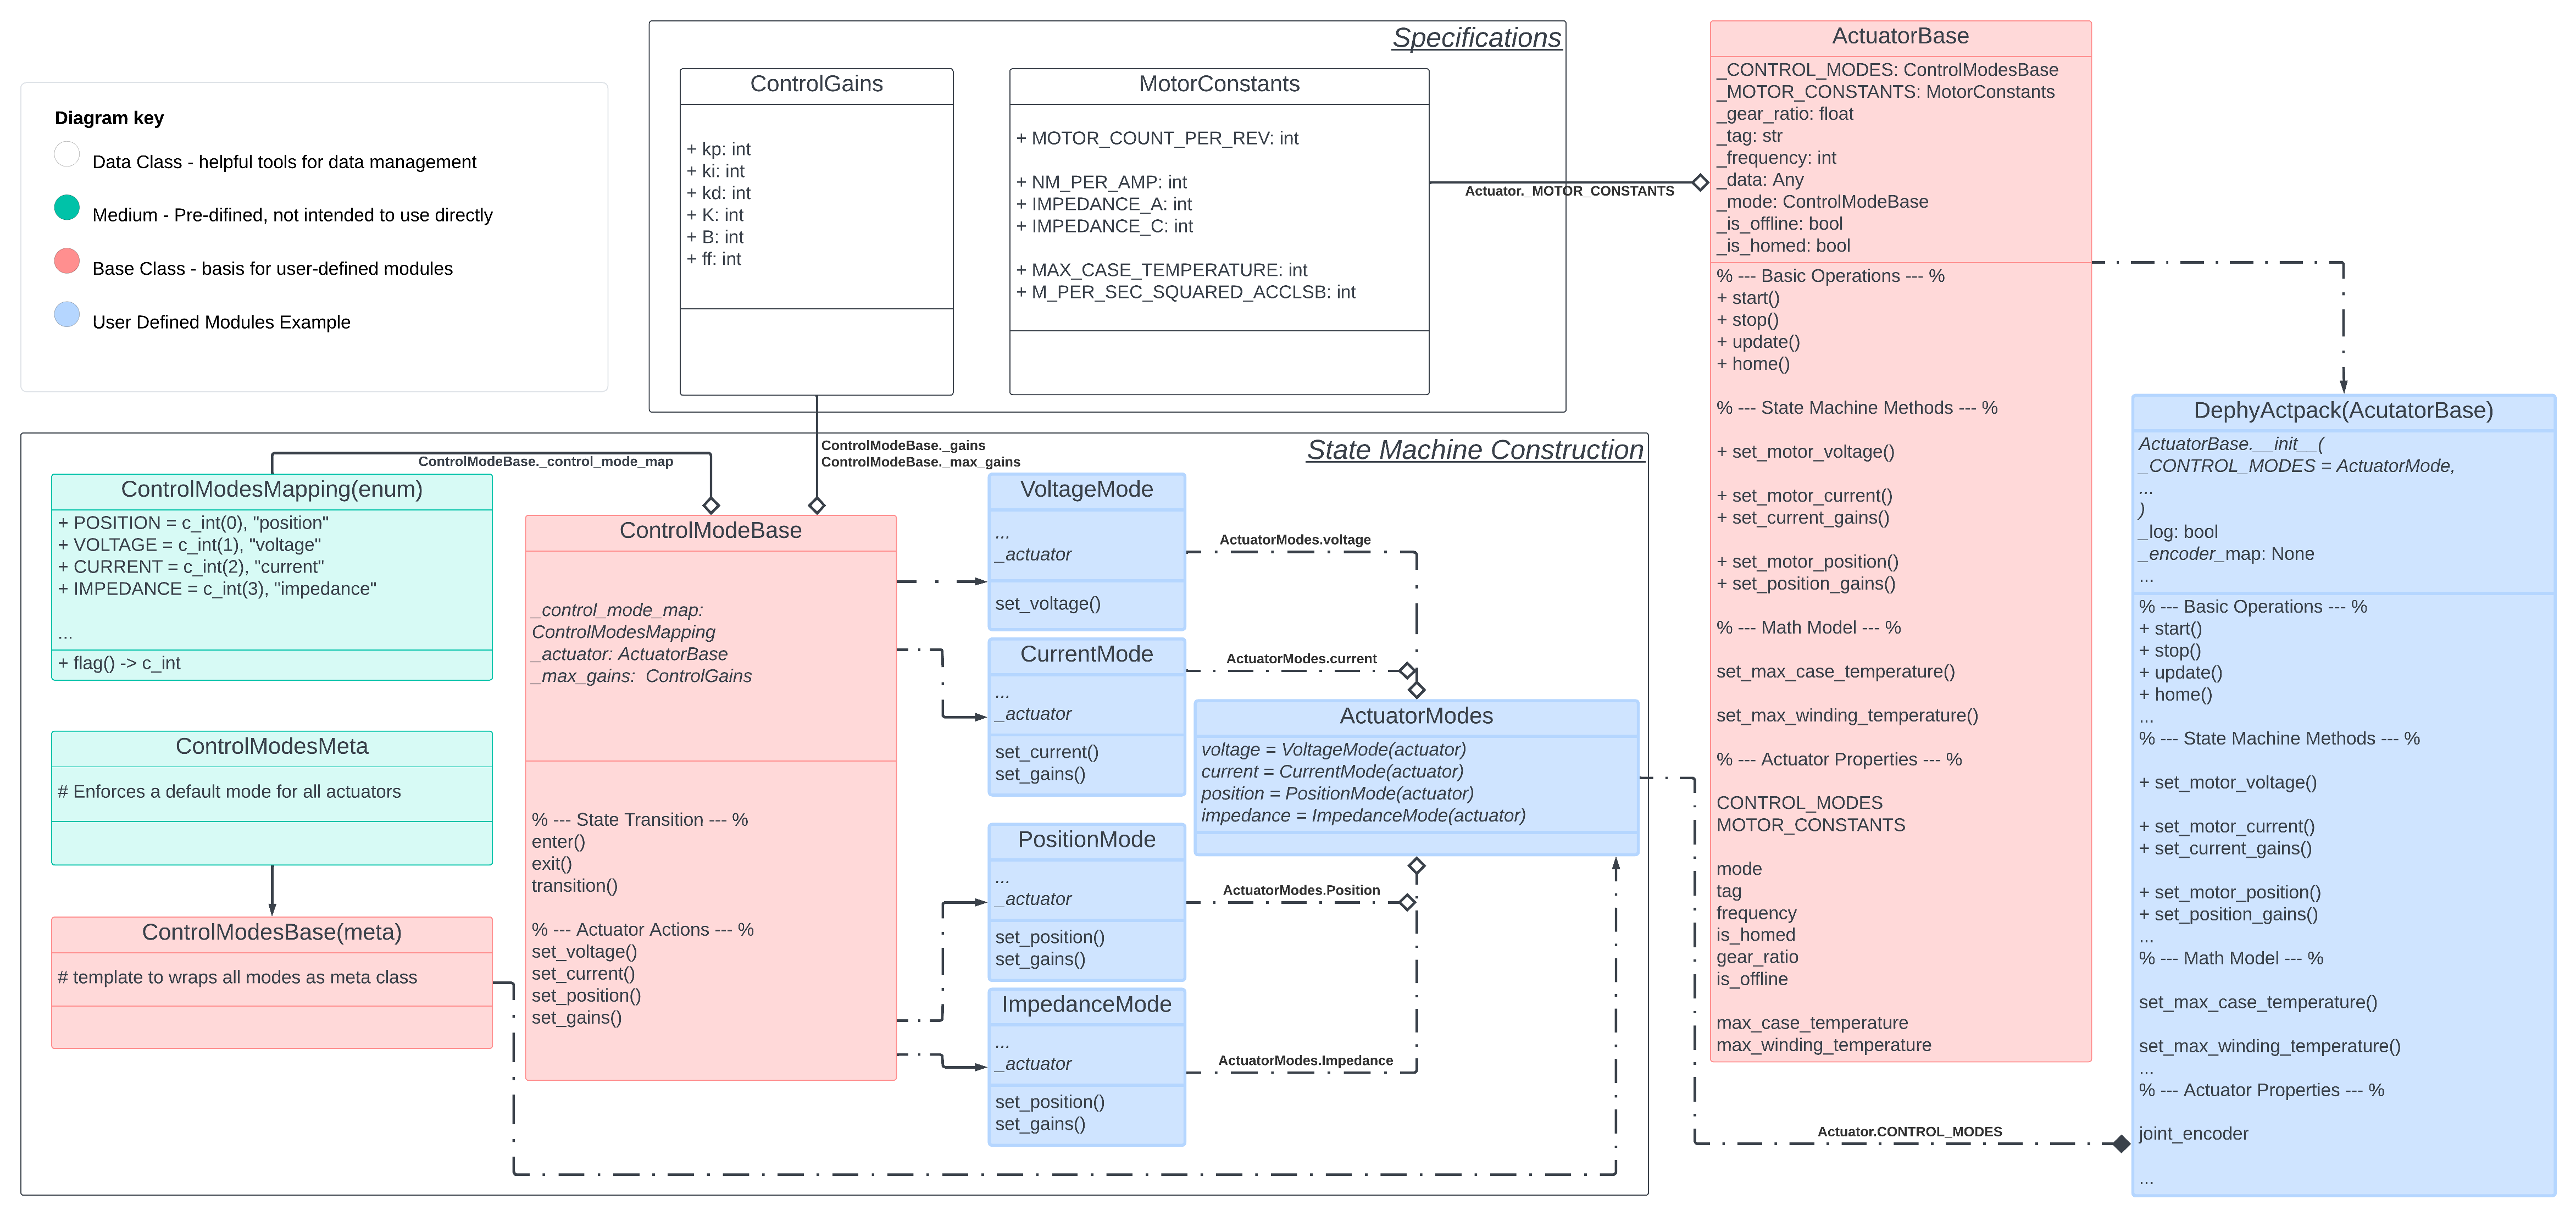
\includegraphics{portfolio/Class Diagram Base Lib.png}

\section{Motion Analysis \& Design of a Robot Swimmer Model}


\subsection{Background}

\subsection{Objectives}

\subsection{Results}


\section{Automated Vehicle with Tracking System}


\subsection{Background}

\subsection{Objectives}

\subsection{Results}


\section{Classification Model Development for Heart Diseases}


\subsection{Background}

\subsection{Objectives}

\subsection{Results}

% -- END OF DOC -- % 
\end{document}